% !TEX TS-program = xelatex
\documentclass[12pt,a4paper]{article}
\usepackage[section]{placeins} % keep floats within their section

% --- Language & page ---
\usepackage[english]{babel}
\usepackage[a4paper,margin=2.5cm]{geometry}

% --- Fonts (XeLaTeX) ---

% --- Formatting helpers ---
\usepackage{xurl}
\usepackage{enumitem}
\usepackage{setspace}
\setstretch{1.5}
\setlength{\parindent}{0pt}

% --- Graphics ---
\usepackage{graphicx}

% Load caption BEFORE subcaption; set “Figure 1.” (period, not colon)
\usepackage{caption}
\captionsetup{
  labelsep=period,
  labelfont=bf,
  textfont=normalfont}

\usepackage{subcaption}

% Subfigure labels: a b c (no parentheses), above, top-left
\renewcommand\thesubfigure{\alph{subfigure}}
\captionsetup[subfigure]{
  labelformat=simple,
  labelsep=space,
  position=above,
  justification=raggedright,
  singlelinecheck=false,
  labelfont=bf
}
% --- Links (load before biblatex) ---
\usepackage{hyperref}
\hypersetup{colorlinks=true, linkcolor=blue, urlcolor=blue, citecolor=blue}

% --- Bibliography (biber) ---
\usepackage[backend=biber,style=authoryear,sorting=nyt]{biblatex}
\addbibresource{Citations.bib}
\usepackage{csquotes}

% --- Underscore in text/URLs without breaking ---
\usepackage[strings]{underscore}
\usepackage{fontspec}
\setmainfont{Times New Roman}

% --- Headers/footers ---
\usepackage{fancyhdr}
\pagestyle{fancy}
\fancyhf{}
\fancyfoot[C]{\thepage}

% --- Diagnostics ---
\overfullrule=0pt
\begin{document}

% ===========================
%   TITLE PAGE
% ===========================
\begin{center}
	\hrule
	\vspace{0.5cm}

	{\Large \textbf{
			Computergestützte Inferenz und Analyse von PRDM9-unabhängigen meiotischen
			Rekombinations-Hotspots in Populationen der Europäischen Mönchsgrasmücke
			\textit{Sylvia atricapilla}}}\\[0.5cm]

	{\large Computational inference and analysis of prdm9 independent meiotic
	recombination hotspots in European Blackcap \textit{Sylvia atricapilla} populations}\\[0.5cm]

	\hrule
	\vspace{0.5cm}

	\textbf{Masterarbeit}\\[2pt]
	im Ein Fach Masterstudiengang\\
	Fach Molekulare Biologie und Evolution\\
	der Mathematisch Naturwissenschaftlichen Fakultät\\
	der Christian Albrechts Universität zu Kiel\\[0.5cm]

	\textit{Master's thesis}\\[2pt]
	in the single-subject Master's program\\
	subject Molecular Biology and Evolution\\
	of the Faculty of Mathematics and Natural Sciences\\
	of the Christian-Albrechts-University of Kiel\\[0.5cm]
	\hrule
	\vspace{0.5cm}
	vorgelegt von\\
	\textbf{Orion Pirku}\\[6pt]
	\textit{submitted by}\\
	Orion Pirku\\[0.5cm]

	\hrule
	\vspace{0.5cm}
	Erstgutachter: Dr. Linda Odenthal-Hesse\\
	Zweitgutachter: Prof. Dr. Eva Stukenbrock\\[0.5cm]

	\hrule
	\vspace{0.5cm}
	Kiel, Deutschland \quad 11/2025\\
	\textit{Kiel, Germany \quad 11/2025}

\end{center}
\newpage
%=============================
%   TABLE OF CONTENTS
%=============================
\pagenumbering{arabic}
\tableofcontents
\newpage
%=============================
%   MAIN DOCUMENT
%=============================
\section{Introduction}
%=============================
%   MATERIALS AND METHODS
%=============================
\section{Materials \& Methods}
\subsection{Data Acquisition}
To computationally identify and characterize prdm9-independent hotspots in
European blackcap (\textit{Sylvia atricapilla}), hereafter referred to as
blackcap, on 15 March 2025 I retrieved:
\begin{itemize}[label=--,itemsep=0pt]
	\item Population level blackcap whole genome variant call \texttt{VCF}, blackcap
	      individual identifiers and inferred demography history data through SMC from
	      \parencite{ishigohoka_high-recombining_2025}.
	\item Blackcap genome assembly, \texttt{GFF} and genome sizes from NCBI with genome
	      accession number \texttt{GCF\_009819655.1} \parencite{NCBI}.
	\item Zebra finch to blackcap lift-over chain file
	      \texttt{taeGut2ToGCF\_009819655.1.over.chain} from the UCSC genome browser
	      \parencite{UCSC, UCSC_2006_LiftOver}.
	\item Zebra finch recombination rate maps from \cite{singhal_2015}
\end{itemize}
As the demography data from \cite{ishigohoka_high-recombining_2025} was computed for each blackcap
sub population, I merged the msmc2 table by taking the average of each input across all tables.
I automated this process with a custom script \texttt{merge\_msmc2\_table.py}.
\subsection{Population Genomics Statistics}
To describe the different aspects of genomic variation, such as average pairwise sequence
variation between individuals, frequency of polymorphic sites and deviation from natural evolution I
computed key population genomics statistics: \textbf{Tajima's D},
\textbf{Window $\pi$} and \textbf{SNP density} using \texttt{VCFTools}
(v0.1.16) \parencite{vcftools, Tajima-1989, nei-and-li-1979}. To compute the statistics I first sampled 100
random individual identifiers using \texttt{GNU shuf} and saved them into a
file called \texttt{n100\_blackcap.panel}. Using this file, I then extracted
the corresponding SNP records with a minor allele frequency \texttt{maf} of
0.05\% and computed the statistics in window sizes of 1000, 5000, 10,000 and
100,000 base pairs (bp). Next, I plotted the genome-wide distribution of each
statistic against their midpoints, which where calculated through the formula:
$\frac{Start + End}{2}$ \\ Lastly, divided the statistics into three equal
quantile-based bins representing "low", "medium" and "high" values and
visualized the proportion of each quantity per chromosome. I automated the
visualization with a custom script called \texttt{plot\_popgen\_stats.py}.
\subsection{Inference of Recombination Rate Maps}
To compute the population scaled recombination rate maps in blackcaps, I
utilized a demography- aware method to infer fine-scale recombination rates
between SNPs called \texttt{pyrho} \parencite{doi:10.1126/sciadv.aaw9206}. I
first precomputed the likelihood tables using \texttt{pyrho make\_table} needed
for estimating the population-specific recombination rate
\parencite{doi:10.1126/sciadv.aaw9206}. The table was precomputed with the
following parameters:
\begin{itemize}[label=--, itemsep=0pt]
	\item Mutation rate $\mu: 4.6\times10^{-9}$, as reported in
	      \cite{bascon-cardozo-fine-scale-2024}
	\item Decimal relative tolerance: 0.1 as reported in
	      \cite{bascon-cardozo-fine-scale-2024}
	\item Population size (i.e., number of haplotypes): 200
	\item Moran population size: 200
	\item The averaged MSMC2 demography history data.
\end{itemize}
I automated this process with a custom script, \texttt{make\_table.sh}. Secondly, I optimized
the \texttt{block penalty} and \texttt{window size}, two hyper\-parameters' required for
the computation of the population\-scaled recombination rate, using \texttt{pyrho hyperparam}
\parencite{doi:10.1126/sciadv.aaw9206}. I ran 10 simulations over the following grid of values:
\begin{itemize}[label=--, itemsep=0pt]
	\item \textbf{Block Penalty}: 10, 20, 30, 40, 50
	\item \textbf{Window Size}: 25, 30, 50, 100, 1000
\end{itemize}
The optimization used the Averaged MSMC2 demography history and precomputed likelihood table
from the previous step. This step was automated using \texttt{optimize\_hyperparameters.sh}.
\texttt{pyrho hyperparam} returns a table with the pearson and spearman correlation coefficients
and the $L2$ norm. I selected a \textbf{window size of 100} with a \textbf{block penalty of 20} as they maximized
the pearson and spearman correlation coefficient while minimizing the $L2$ norm,
as specified by \parencite{doi:10.1126/sciadv.aaw9206}. I sampled the same 100 individuals from
the \texttt{VCF} data as in section 2.2, but only with allele count of at least 2.
Lastly, using the precomputed likelihood, sampled individual SNP data table, window size of 100
with a block penalty of 20 I computed population\-scaled the recombination rate with
\texttt{pyrho optimize} \parencite{doi:10.1126/sciadv.aaw9206}.
This process was automated with a custom script called \texttt{pyrho\_optimize.sh}

\subsection{Analysis of Recombination Rate Landscape Over The Blackcap Genome}
To investigate the population scaled recombination rate landscape in blackcaps,
I converted the raw recombination rate to \texttt{cM/Mb} by averaging over
genomic windows of 10 kilobases and multiplying by $10^8$. Then, I calculated
the midpoint of the genomic coordinates by the formula: $\frac{Start +
		End}{2}$. Lastly, I plotted the recombination rate in \texttt{cM/Mb} over the
genomic midpoint coordinates. \\section I investigated the distribution of
recombination rate strength per chromosome. To do this, I sorted the
recombination rate per chromosome by signal strength and divided it into equal
tertiles ("low", "medium" and "high"). I visualized the data on a chromosomal
basis using pie charts. \\

To gain a more in\-depth understanding of the recombination landscape I
incorporated the gene density and gc content into the analysis. I extracted the
genes from the blackcap \texttt{gff} file using a custom script
\texttt{clean\_raw\_gff.py} and computed the gene density over genomic windows
ofsize $n$. I generated genomic bins of size $n$ using \texttt{PyRanges},
counted the number of genes overlapping with each window and divided by the
window size and plotted the distribution of the gene density along the genome
and binned the gene density into tertiles representing "low", "medium" and
"high" to see the proportion To compute the gc content, I used \texttt{bedtools
	makewindows} to make genomic windows per each chromosome, \texttt{bedtools nuc}
to compute the gc content over the windows, which I automated with the script
\texttt{compute\_gc\_content.sh}. Next, I plotted the gc content over each
chromosome and binned it into three tertiles ("low", "medium" and "high")
values to visualize how the gc content is distributed over the genome. I
automated the plotting in the steps above using the script
\texttt{plot\_popgen\_stats.py} \\

To quantify the correlation between the population genomic statistics, gc
content, gene density and the recombination rate I first intersected each
feature with one another using \texttt{pyRanges}, computed the pearson
correlation coefficient between each genomic feature using \texttt{SciPy} and
visualized the results in a heatmap \parencite{2020SciPy-NMeth}.I automated
this analysis with a custom script called
\texttt{compute\_feature\_correlation.py}. \\

Lastly, I investigated the average profile of the recombination rate over
genomic features (UTR's, CDS, Exons, Intergenic Regions and Genes), which I
extracted from the blackcap \texttt{GFF} using the \texttt{clean\_raw\_gff.py}.
I used deeptool's \texttt{computeMatrix} to calculate the average profile of
the recombination rate over these regions and \texttt{plotHeatmap} to plot the
average profile and heatmap. The average recombination rate profile was
computed for $\pm$ 20 kb and zeros were not reported. The script for computing
the matrix and plotting the profile are:
\texttt{computeRhoMatrix.sh} and
\texttt{plotHeatmap.sh}, respectively.

\subsection{Inference of Meiotic Recombination Hotspots}
To call recombination hotspots from recombination rate maps, I applied
\textbf{Continious Wavelet Transform (CWT)} to detect multi-scale peaks in the
signal. To do so the wavelet is continiously rescaled accross a grid of
specified scales and shifted along the signal, producing coefficients that
quantify local similarity between the signal and the wavelet shape at each
position and scale. The higher the similarity, the higher coefficients
\parencite{Singh2022, Mexican-hat-wavelet}. Before computing the cwt with
\texttt{PyWavelet}, I smoothed the recombination rate $\rho$ signal using
\texttt{SciPy's} one dimensional gaussian filter (\texttt{gaussian_filter1d})
($\sigma = 5$) to remove excessive high frequency noise. Then, I generated 200
logarithmically spaced scales betweem 50 and 600. With an recombination rate
genomic range of 22 bp this corresponds to genomic bin size between $\sim$ 1.1
kb to $\sim$ 13.2 kb. After computing the wavelet coefficients, I normalized
the coefficients at each scale independently through \texttt{z-score}.
Following this, I selected only those coefficients, which had a z-score: $z >
	2.0$ and persisted in atleast 30\% of the scales. The peaks were then
identified using SciPy's \texttt{find_peaks} with a minimum peak prominence of
at least the $90^{th}$ percentile. This process was automated using the script
\texttt{find_hotspots.py}. Lastly, I used the package \texttt{cobind.py} to
quantify the amount of overlap between the identified recombination hotspots
and genomic features (UTRs', codons, genes, intergenic regions) \parencite{ma_cobind_2023} \\
To test if the wavelet transform methodology is
also applicable to other prdm9 independent recombining species I ran the same
analysis on \texttt{LDHelmet} recombination maps generated by \cite{singhal_2015}.

\section{Results}
\subsection{Population genomics statistics of the european blackcap metapopulation}
\FloatBarrier
To investigate the deviation from neutral evolution, average pairwise nucleotide diversity and snp
density I computed three population genomics statistics: tajima $D$, diversity \(\pi\) and SNP
density across the autosomal chromosomes on a blackcap metapopulation consisting of 100 individuals.
Tajima's $D$ showed two types of patterns across each of the 33 blackcap autosomal
chromosomes (Figure 1, Supplementary Figure 1). The large chromosomes one through 12, showed
relatively stable negative tajima $D$ values across the chromosomal body, with the exception of one
peak in chromosomes  2 and 4 at \(\sim20 Mb\) with a tajima $D$ value of 0 and a sharp valley with a
tajima $D$ value of over -2 at \(\sim7 Mb\) on chromosome 6, and the end of chromosome 12 that
contained several peaks of positive tajima $D$ (Supplementary Figure 1). The chromosomal ends of
these macrochromosomes had negative tajima $D$ values which were close to 0. \\

The blackcap microchromosomes displayed opposite patterns, the subtelomeric regions had valleys
beyond values of tajima $D:$ $-2$ while the chromosomal body showed stable yet tiny fluctuations in
the tajima $D$ values, which were negative yet closer to 0 (Supplementary Figure 1).
% --- Tajima's D ---
\begin{figure}[htbp]
	\centering
	\begin{subfigure}{0.65\textwidth}
		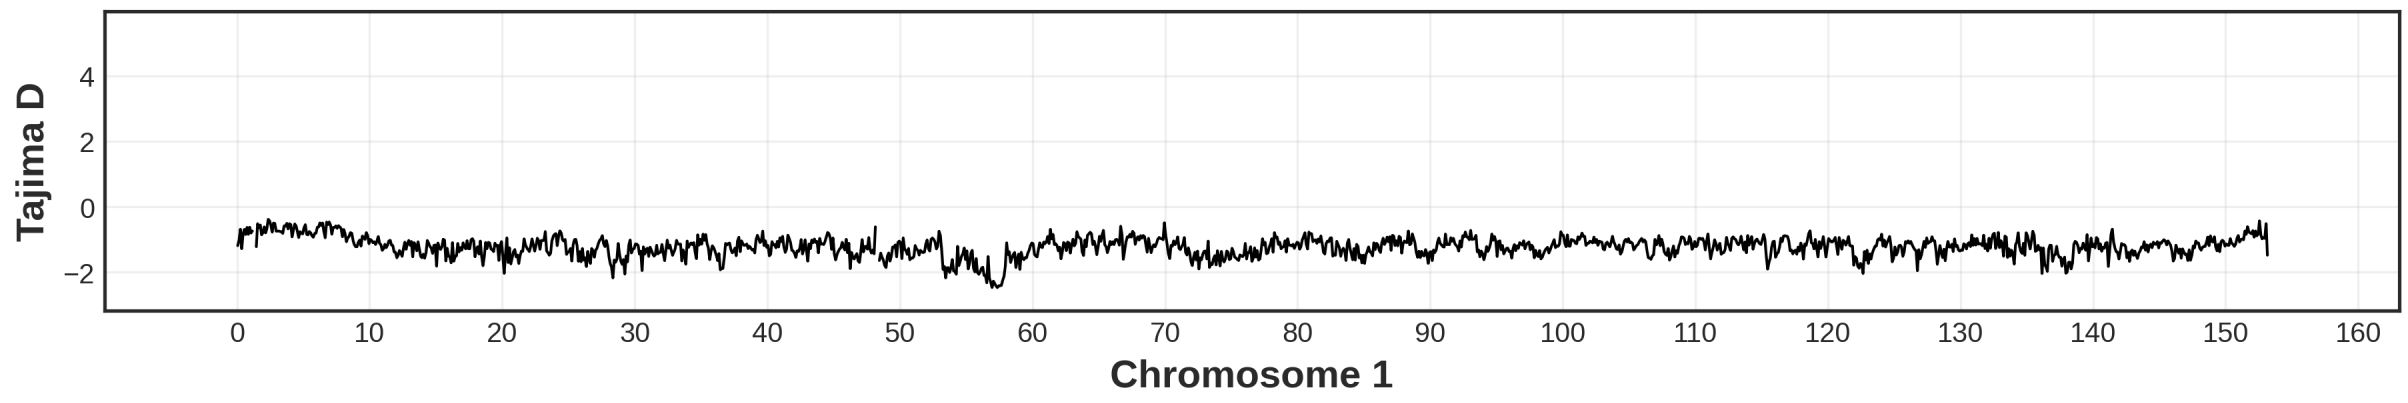
\includegraphics[width=\linewidth]{Figures/TajimaD_chr1.png}
		\subcaption{}
	\end{subfigure}\par\medskip
	\begin{subfigure}{0.65\textwidth}
		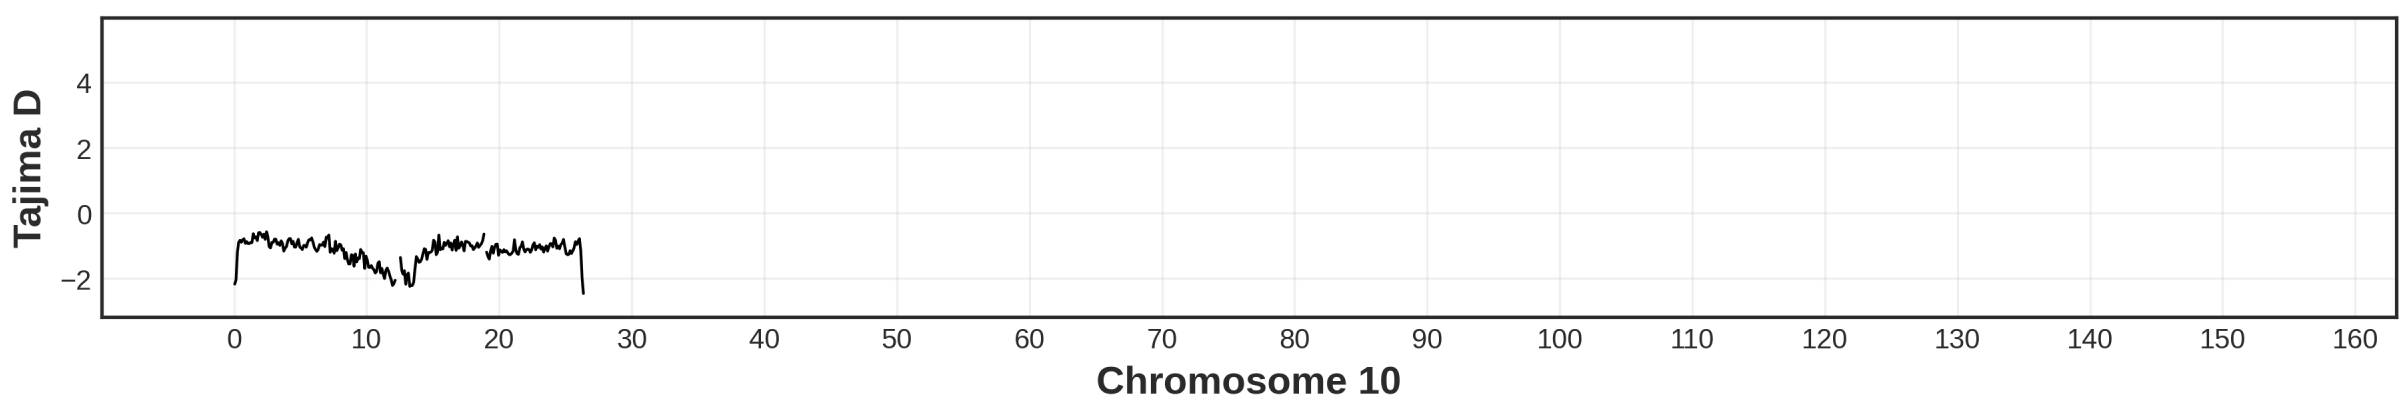
\includegraphics[width=\linewidth]{Figures/TajimaD_chr10.png}
		\subcaption{}
	\end{subfigure}\par\medskip
	\begin{subfigure}{0.65\linewidth}
		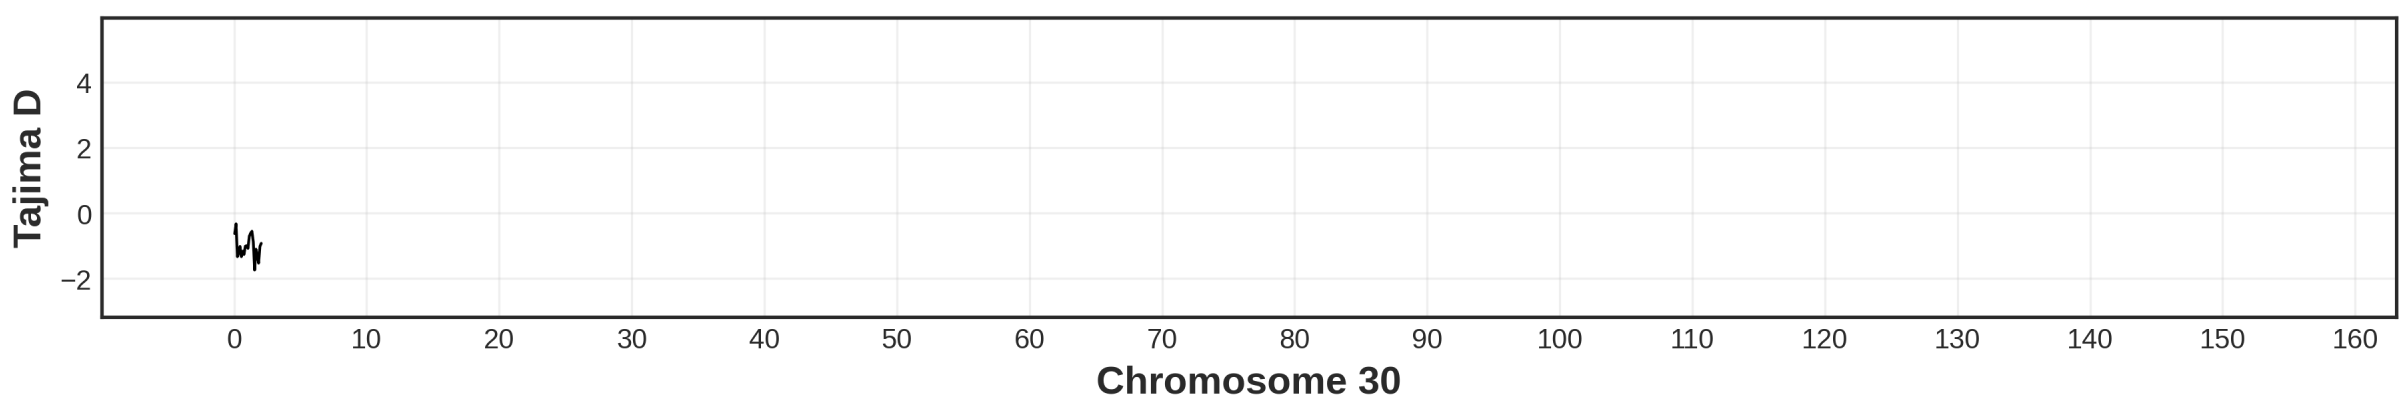
\includegraphics[width=\linewidth]{Figures/TajimaD_chr30.png}
	\end{subfigure}
	\caption{Tajima's \(D\) across chromosomes 1, 10, and 30 in 100\,kb windows for a European
		Blackcap metapopulation (100 individuals from continental and island populations).}
\end{figure}


Compared to tajima's $D$, the SNP density and nucleotide diversity \(\pi\) displayed more visible
patterns across the chromosomes (Figure 2). The macrochromosomes had an average SNP density and
nuleotide diversity \(\pi\) of 50 and 0.005 over 100 Mb window bins, respectively
(Figure 2; Supplementary Figure 2 \& 3). In addition to this, both values displayed  regularly
interspaced sharp valleys occuring at \(\sim\) 10 Mb. Chromosome 1, in contrast to the other,
macrochromosomes had a sharp peak in its chromosomal end (Supplementary Figures 2 \& 3). The
microchromosomes, on the other hand, revealed stable patterns, with reduced signal in the
subtelomeric regions with occasional valleys in SNP density and diversity $\pi$ along the chrmosomal
axis (Supplementary Figures 2\&3). Here again, microchromosomes displayed increased SNP density and

\begin{figure}

	\begin{subfigure}{0.48\linewidth}
		\centering
		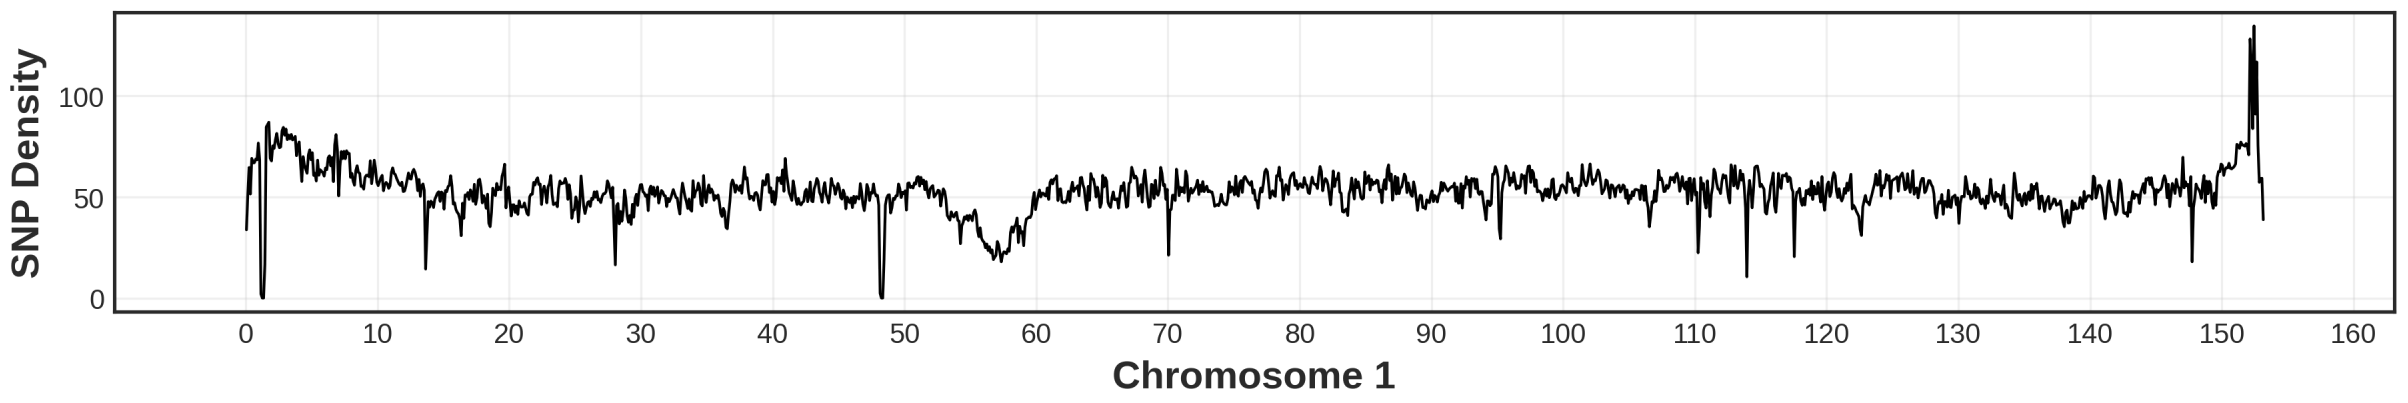
\includegraphics[width=\linewidth]{Figures/SNPDensity_chr1.png}\par\medskip
		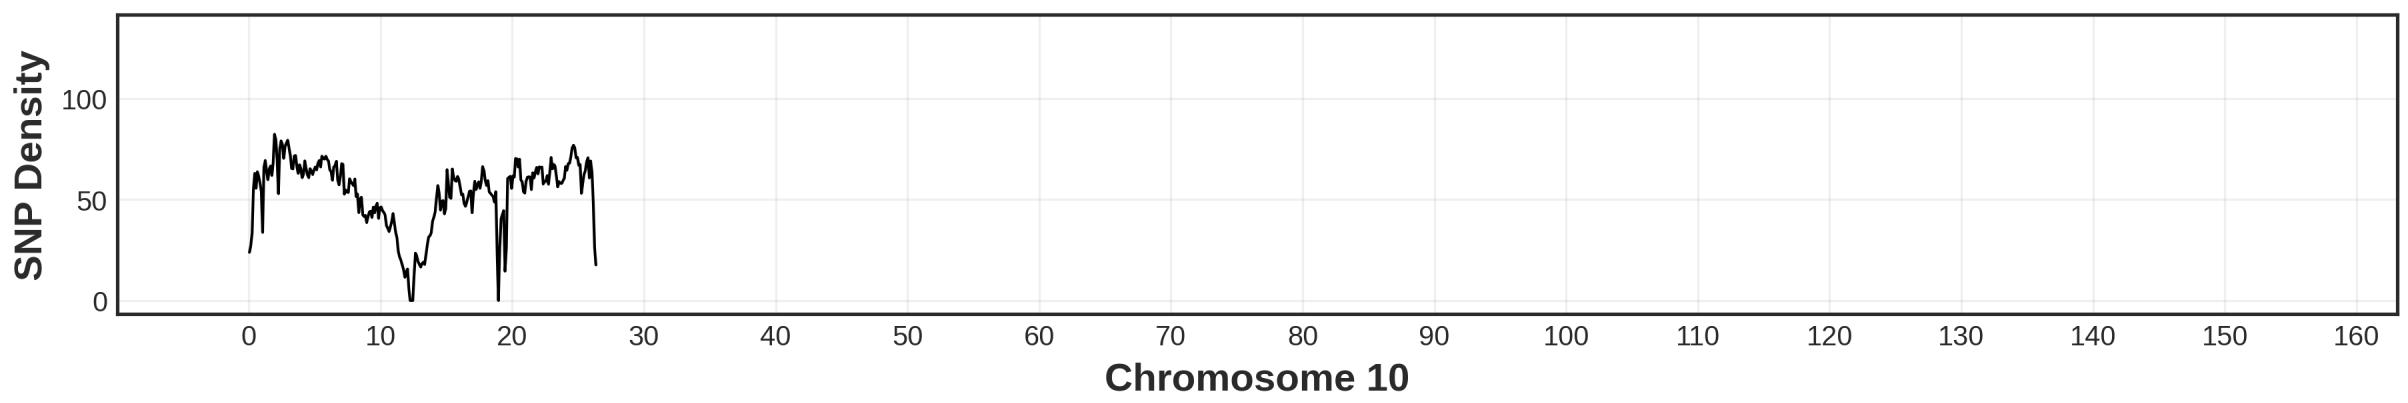
\includegraphics[width=\linewidth]{Figures/SNPDensity_chr10.png}\par\medskip
		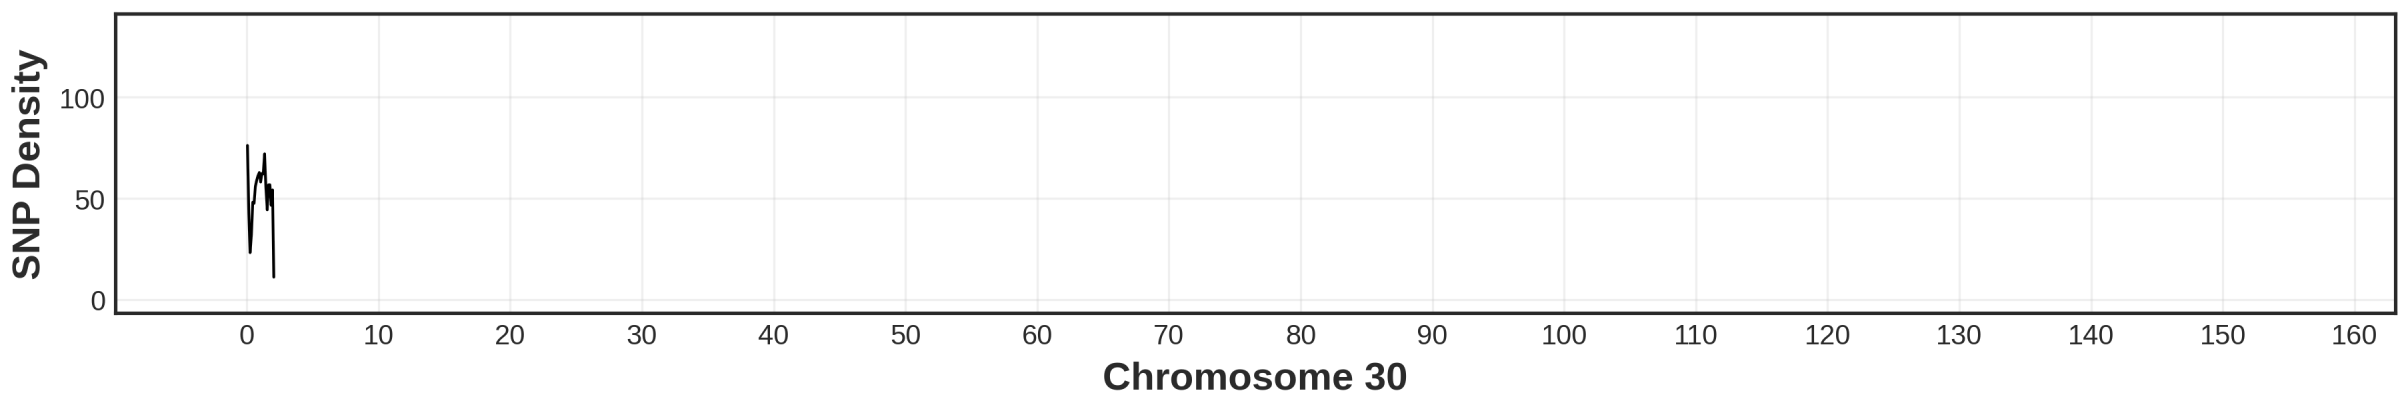
\includegraphics[width=\linewidth]{Figures/SNPDensity_chr30.png}
	\end{subfigure}
	\hfill
	% Right column: Pi
	\begin{subfigure}{0.48\linewidth}
		\centering
		\includegraphics[width=\linewidth]{Figures/WindowPI_chr1.png}\par\medskip
		\includegraphics[width=\linewidth]{Figures/WindowPI_chr10.png}\par\medskip
		\includegraphics[width=\linewidth]{Figures/WindowPI_chr30.png}
	\end{subfigure}

	\caption{SNP density (left) and nucleotide diversity (\(\pi\)) (right) across chromosomes 1, 10,
		and 30 in 100\,kb windows.}
\end{figure}



\begin{figure}[htbp]
	\centering

	% chr1
	\begin{subfigure}[t]{0.74\linewidth}
		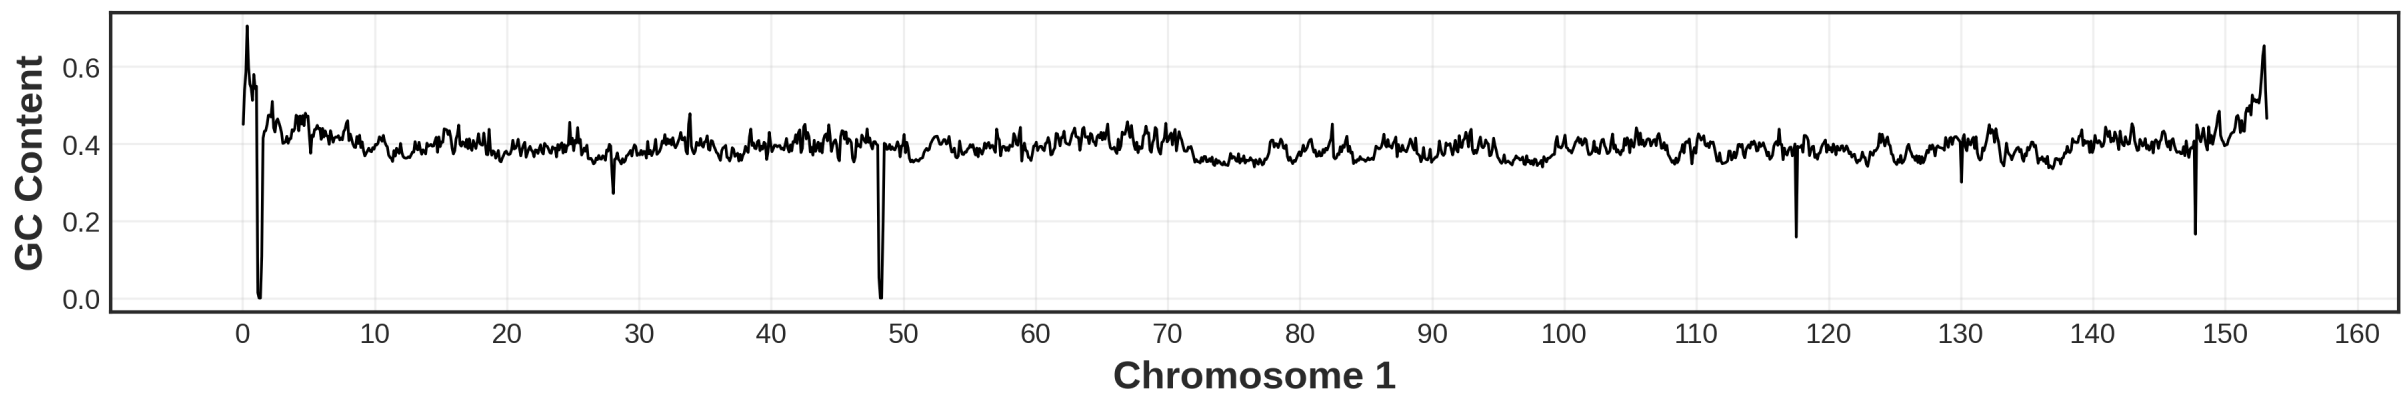
\includegraphics[width=\linewidth]{Figures/GCContent_chr1.png}
	\end{subfigure}\hfill
	\begin{subfigure}[t]{0.24\linewidth}
		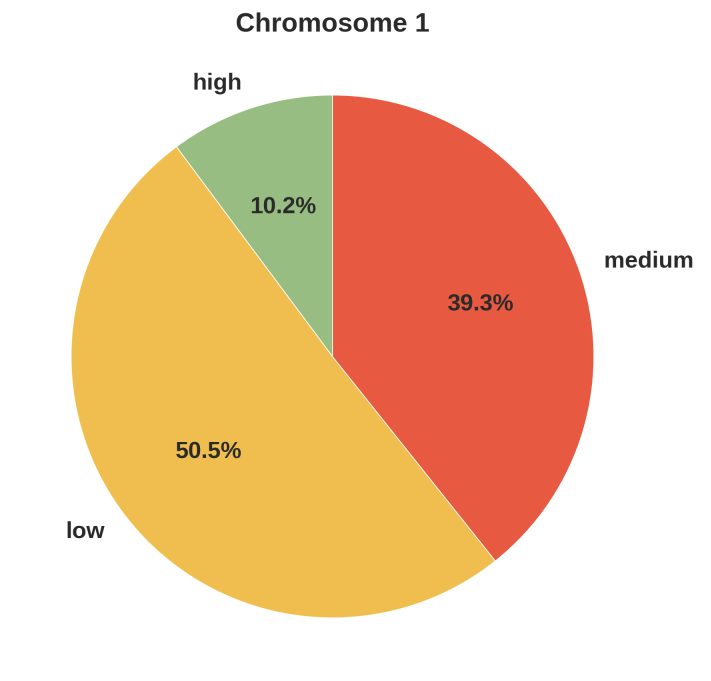
\includegraphics[width=\linewidth]{Figures/GC_dist_chr1.png}
	\end{subfigure}\par\medskip

	% chr10
	\begin{subfigure}[t]{0.74\linewidth}
		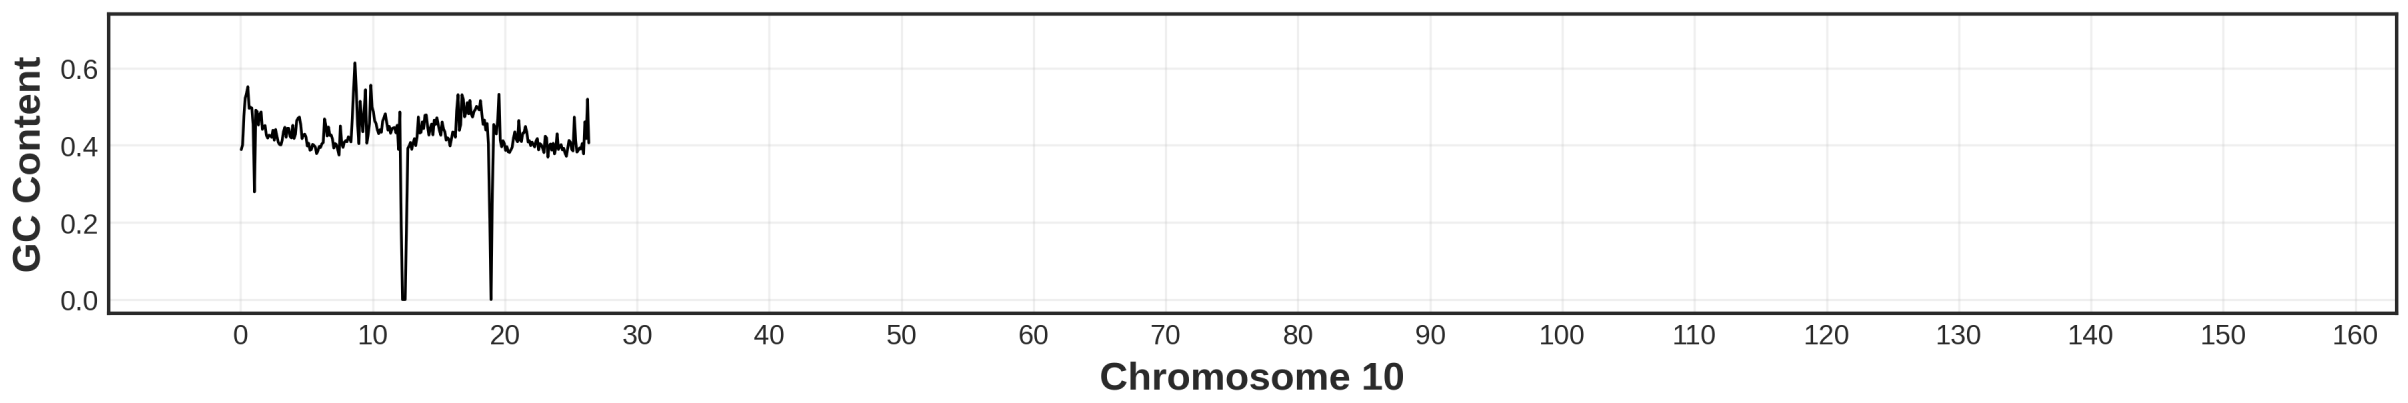
\includegraphics[width=\linewidth]{Figures/GCContent_chr10.png}
	\end{subfigure}\hfill
	\begin{subfigure}[t]{0.24\linewidth}
		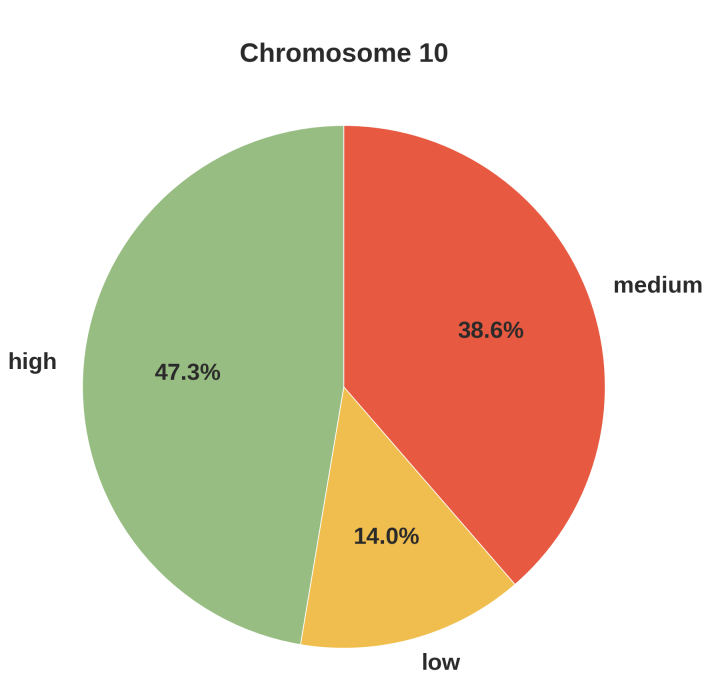
\includegraphics[width=\linewidth]{Figures/GC_dist_chr10.png}
	\end{subfigure}\par\medskip

	% chr30
	\begin{subfigure}[t]{0.74\linewidth}
		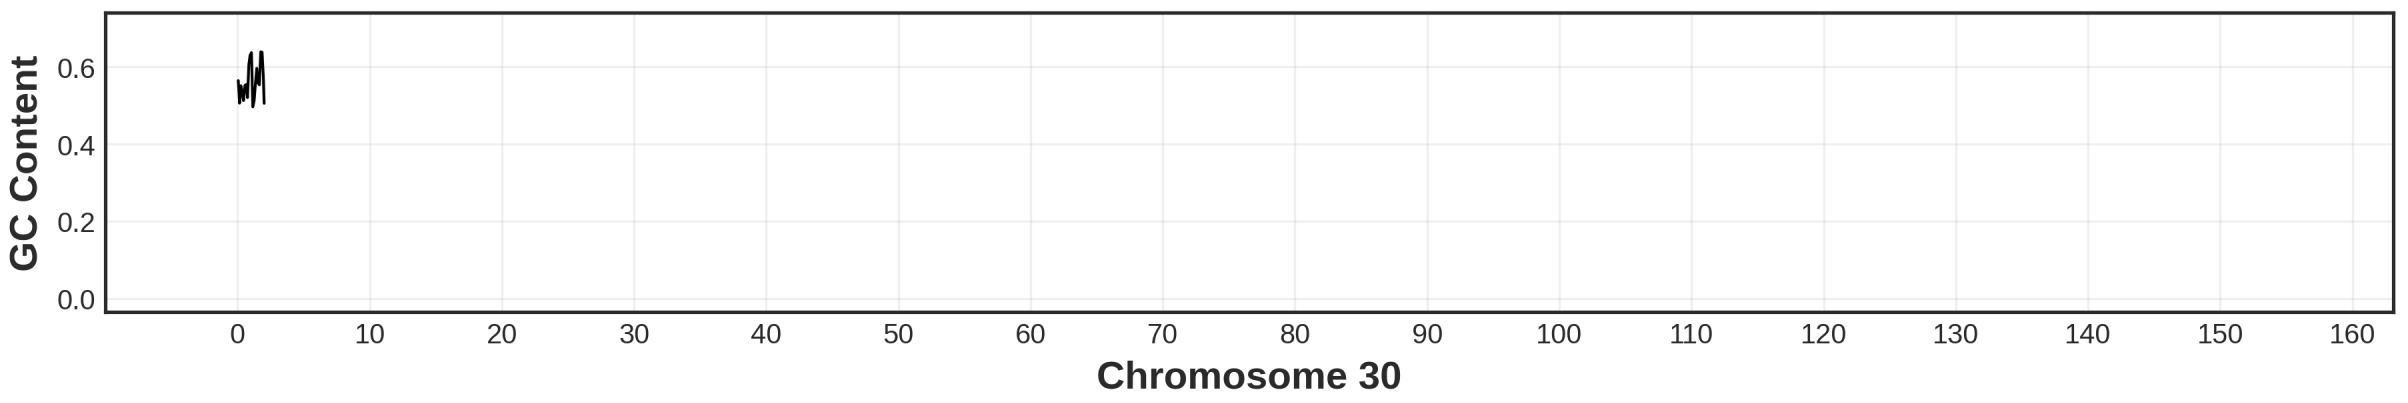
\includegraphics[width=\linewidth]{Figures/GCContent_chr30.png}
	\end{subfigure}\hfill
	\begin{subfigure}[t]{0.24\linewidth}
		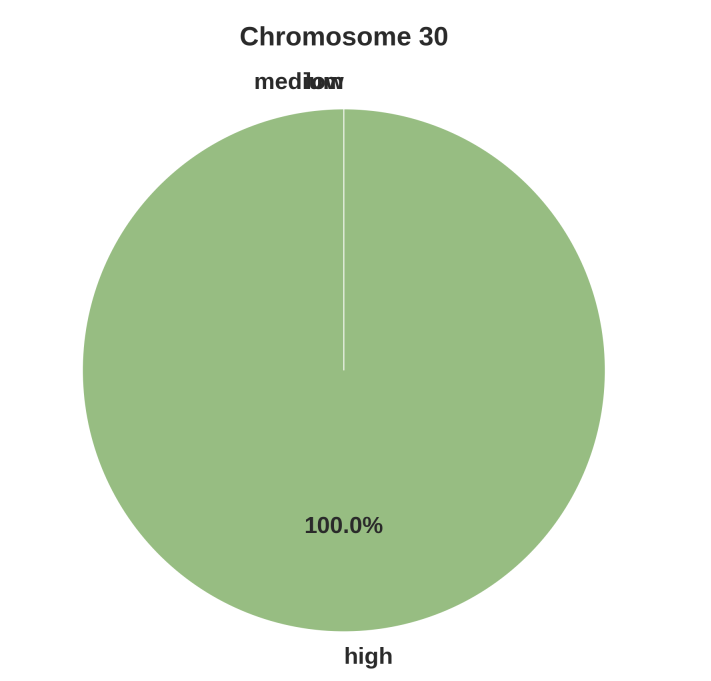
\includegraphics[width=\linewidth]{Figures/GC_dist_chr30.png}
	\end{subfigure}

	\caption{\textbf{(left)} GC content across chromosomes 1, 10, and 30 in 100\,kb windows and
		\textbf{(right)} GC content binned into equal tertiles (\emph{low}, \emph{medium}, \emph{high}).}
\end{figure}

% --- Gene density (tracks + pies) ---
\begin{figure}[htbp]
	\centering

	% chr1
	\begin{subfigure}[t]{0.74\linewidth}
		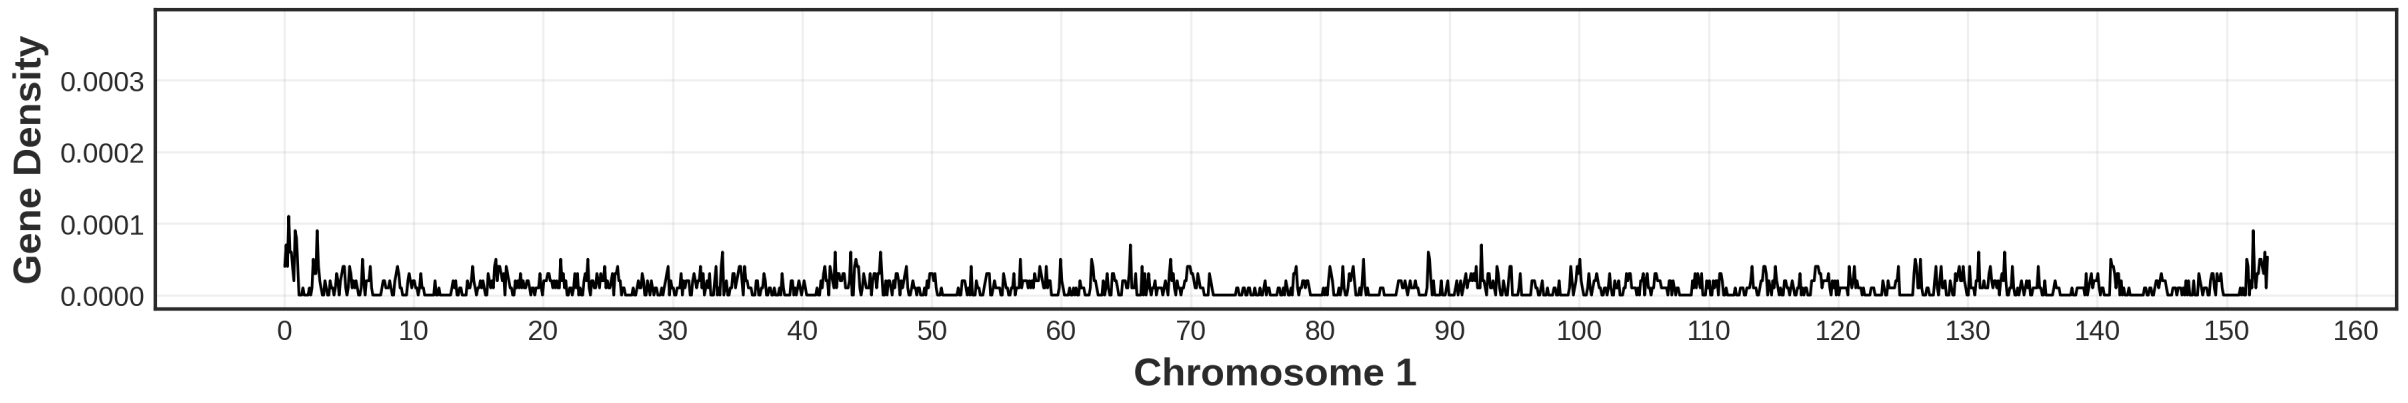
\includegraphics[width=\linewidth]{Figures/GeneDensity_chr1.png}
		\subcaption{}
	\end{subfigure}\hfill
	\begin{subfigure}[t]{0.24\linewidth}
		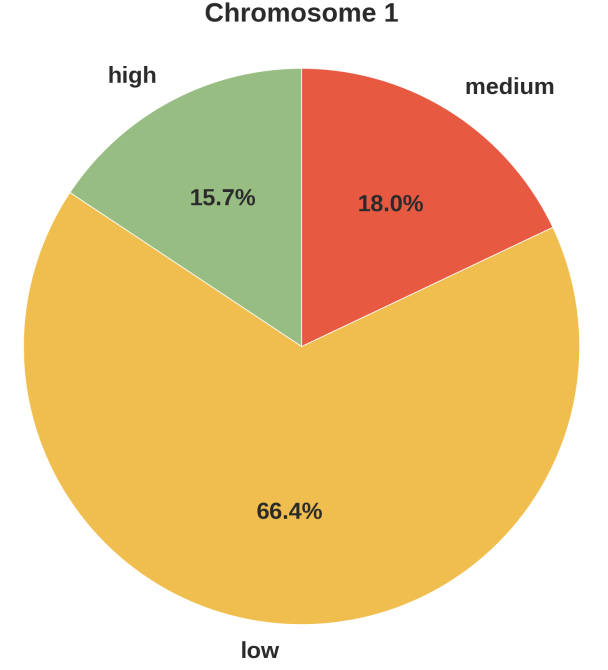
\includegraphics[width=\linewidth]{Figures/GeneDensity_dist_chr1.png}
		\subcaption{}
	\end{subfigure}\par\medskip

	% chr10
	\begin{subfigure}[t]{0.74\linewidth}
		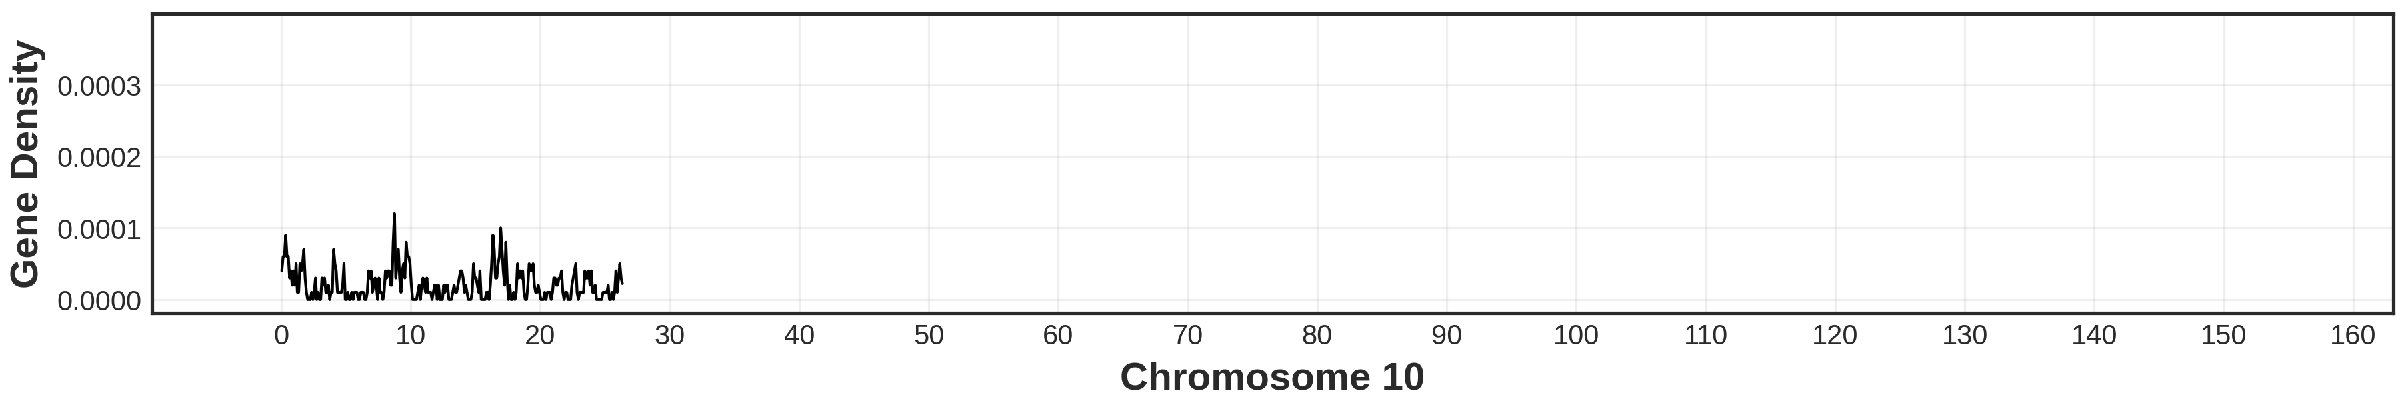
\includegraphics[width=\linewidth]{Figures/GeneDensity_chr10.png}
		\subcaption{}
	\end{subfigure}\hfill
	\begin{subfigure}[t]{0.24\linewidth}
		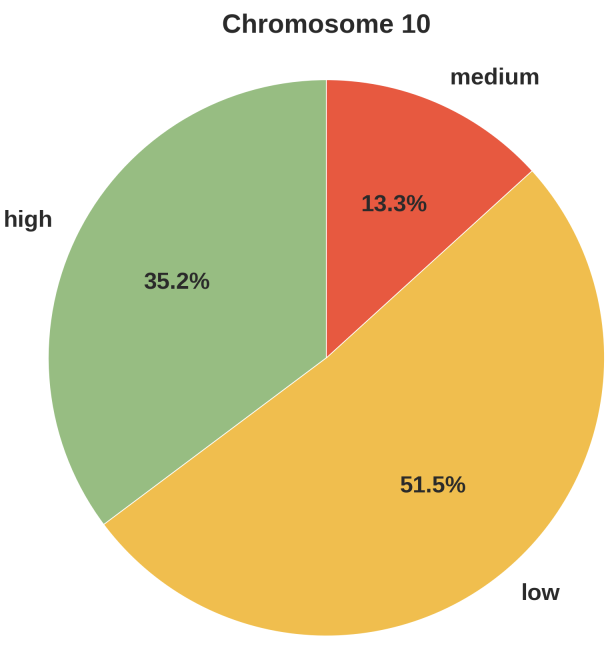
\includegraphics[width=\linewidth]{Figures/GeneDensity_dist_chr10.png}
		\subcaption{}
	\end{subfigure}\par\medskip

	% chr30
	\begin{subfigure}[t]{0.74\linewidth}
		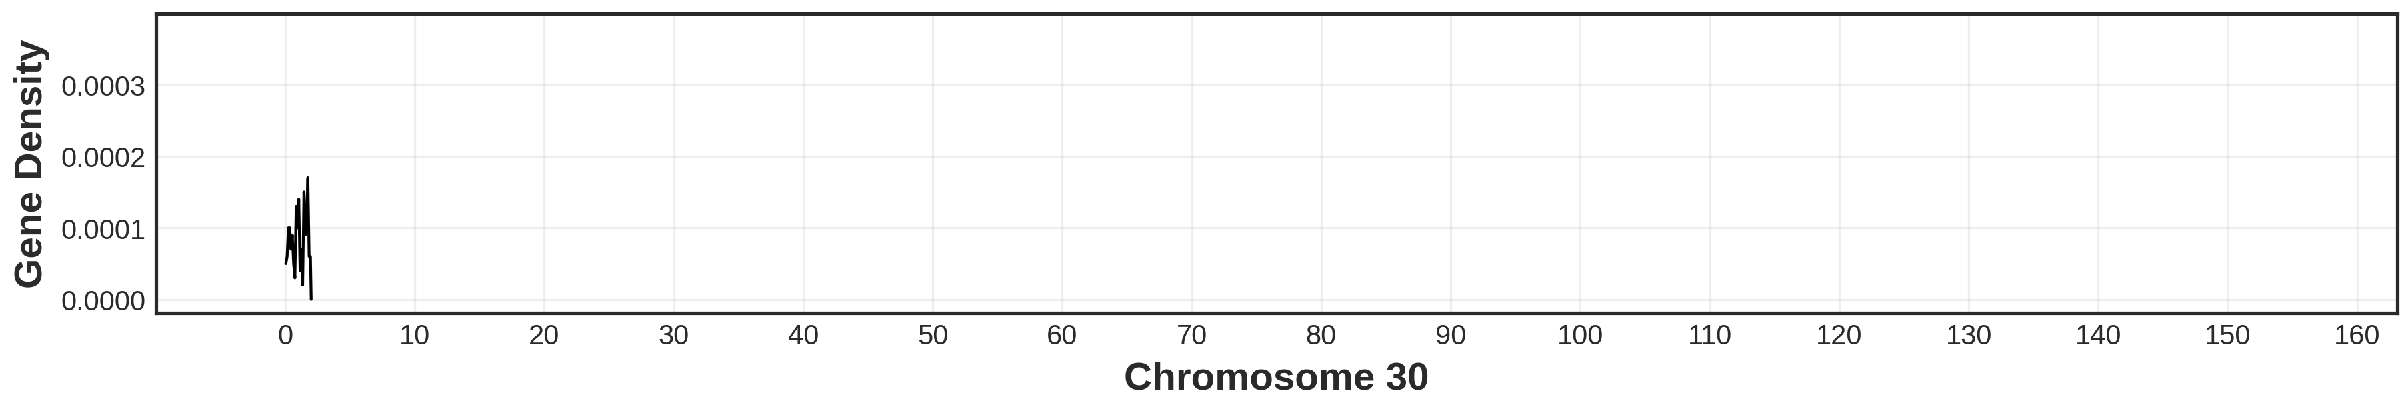
\includegraphics[width=\linewidth]{Figures/GeneDensity_chr30.png}
		\subcaption{}
	\end{subfigure}\hfill
	\begin{subfigure}[t]{0.24\linewidth}
		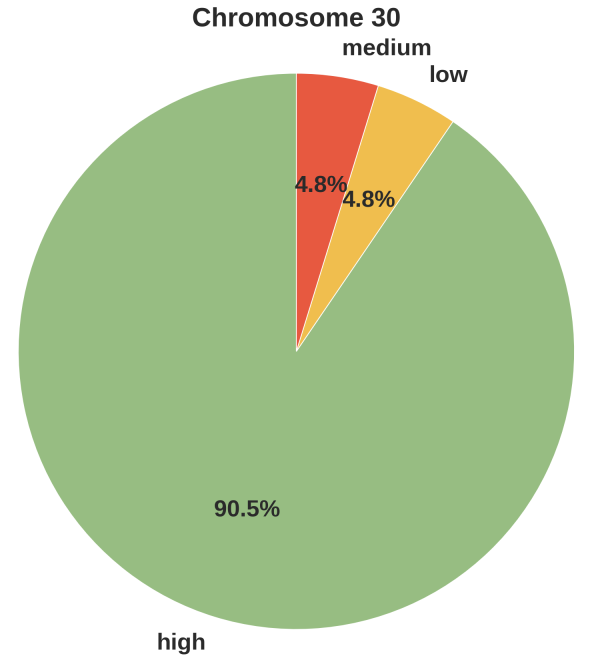
\includegraphics[width=\linewidth]{Figures/GeneDensity_dist_chr30.png}
		\subcaption{}
	\end{subfigure}

	\caption{\textbf{a,c,e}: Gene density across chromosomes 1, 10, and 30 in 100\,kb windows. \textbf{b,d,f}: Gene density binned into equal tertiles (\emph{low}, \emph{medium}, \emph{high}).}
\end{figure}

% --- Gene density (tracks + pies) ---
\begin{figure}[htbp]
	\centering

	% chr1
	\begin{subfigure}[t]{0.74\linewidth}
		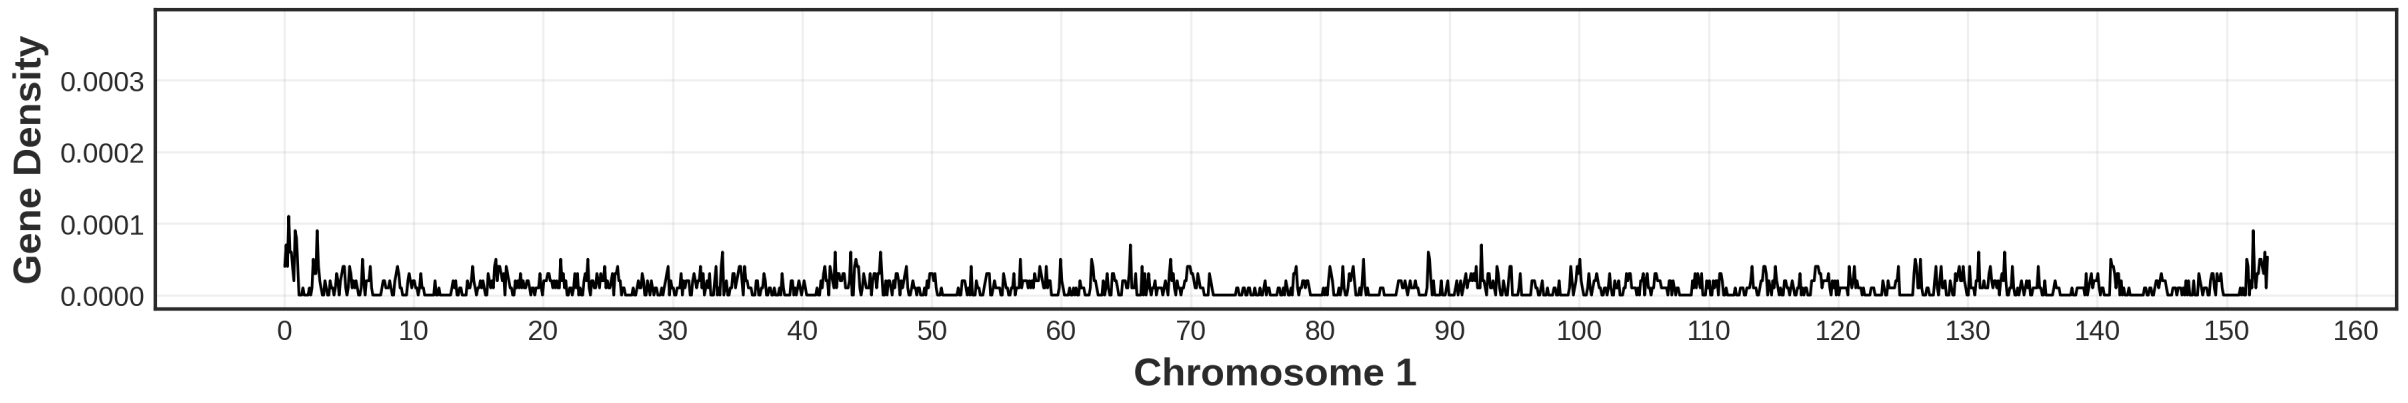
\includegraphics[width=\linewidth]{Figures/GeneDensity_chr1.png}
		\subcaption{}
	\end{subfigure}\hfill
	\begin{subfigure}[t]{0.24\linewidth}
		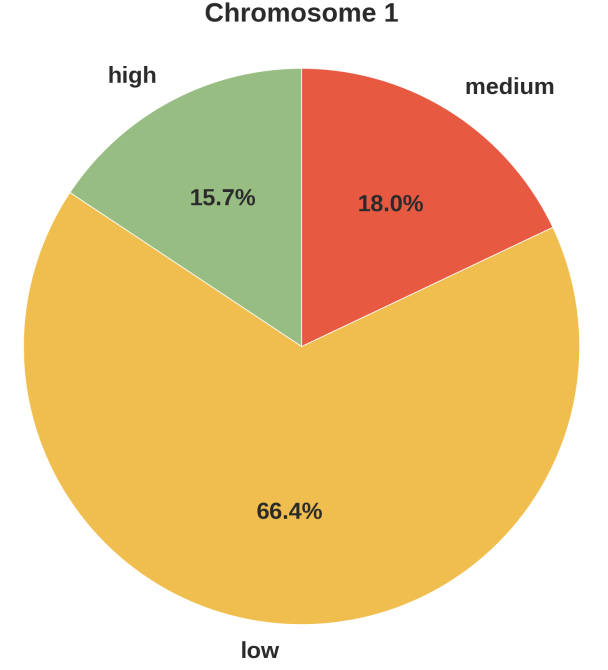
\includegraphics[width=\linewidth]{Figures/GeneDensity_dist_chr1.png}
		\subcaption{}
	\end{subfigure}\par\medskip

	% chr10
	\begin{subfigure}[t]{0.74\linewidth}
		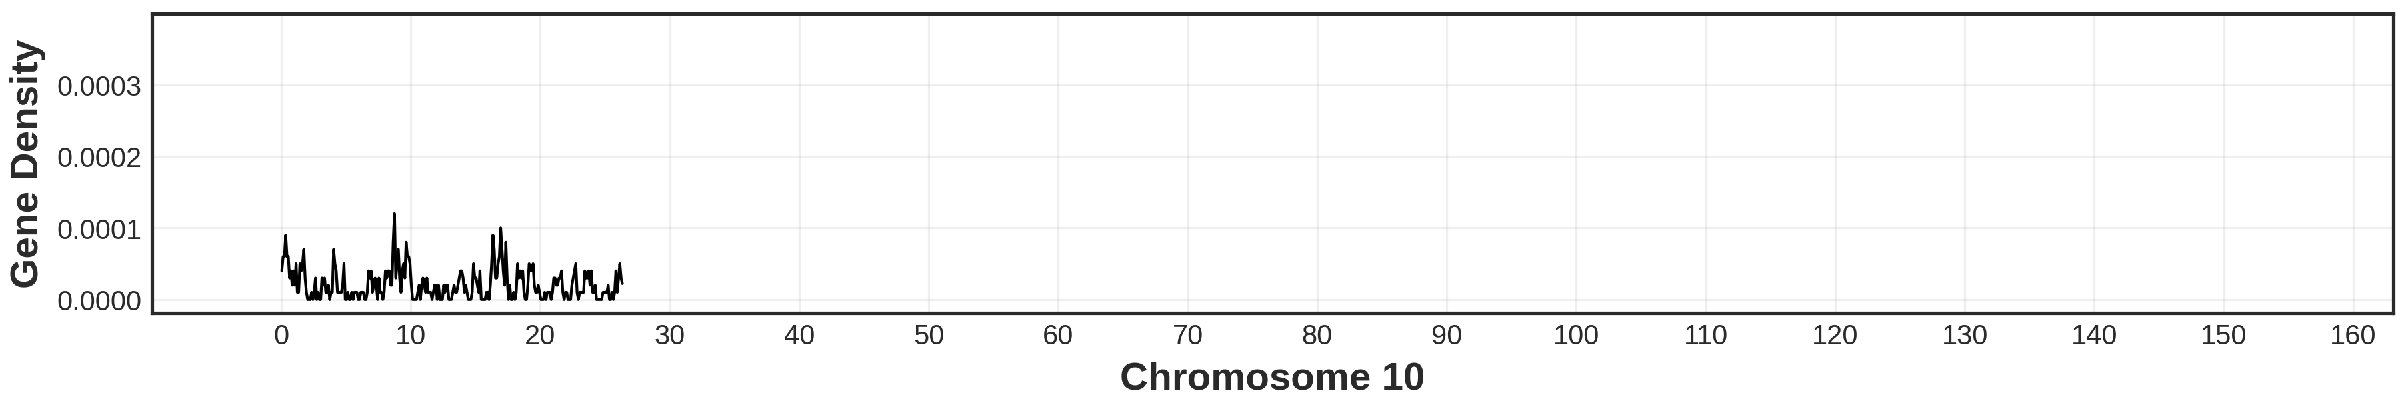
\includegraphics[width=\linewidth]{Figures/GeneDensity_chr10.png}
		\subcaption{}
	\end{subfigure}\hfill
	\begin{subfigure}[t]{0.24\linewidth}
		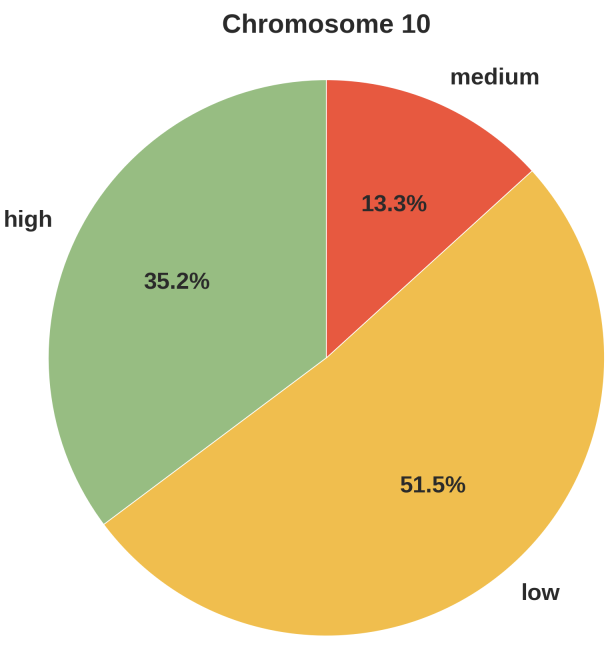
\includegraphics[width=\linewidth]{Figures/GeneDensity_dist_chr10.png}
		\subcaption{}
	\end{subfigure}\par\medskip

	% chr30
	\begin{subfigure}[t]{0.74\linewidth}
		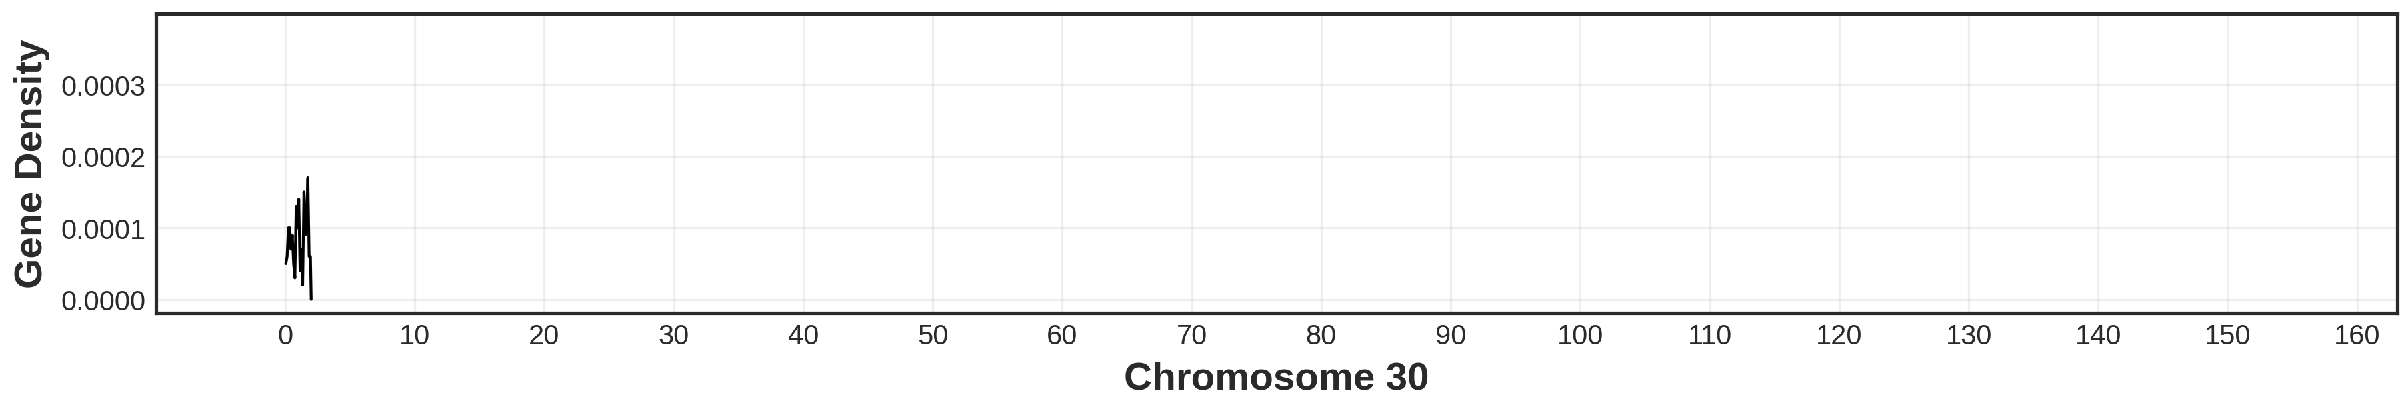
\includegraphics[width=\linewidth]{Figures/GeneDensity_chr30.png}
		\subcaption{}
	\end{subfigure}\hfill
	\begin{subfigure}[t]{0.24\linewidth}
		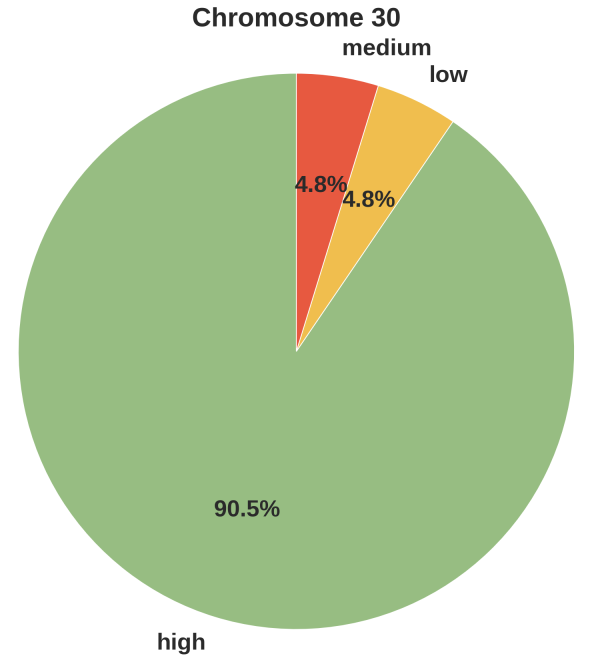
\includegraphics[width=\linewidth]{Figures/GeneDensity_dist_chr30.png}
		\subcaption{}
	\end{subfigure}

	\caption{\textbf{a,c,e}: Gene density across chromosomes 1, 10, and 30 in 100\,kb windows. \textbf{b,d,f}: Gene density binned into equal tertiles (\emph{low}, \emph{medium}, \emph{high}).}
\end{figure}



\begin{figure}[htbp]
	\centering

	% chr1
	\begin{subfigure}[t]{0.74\linewidth}
		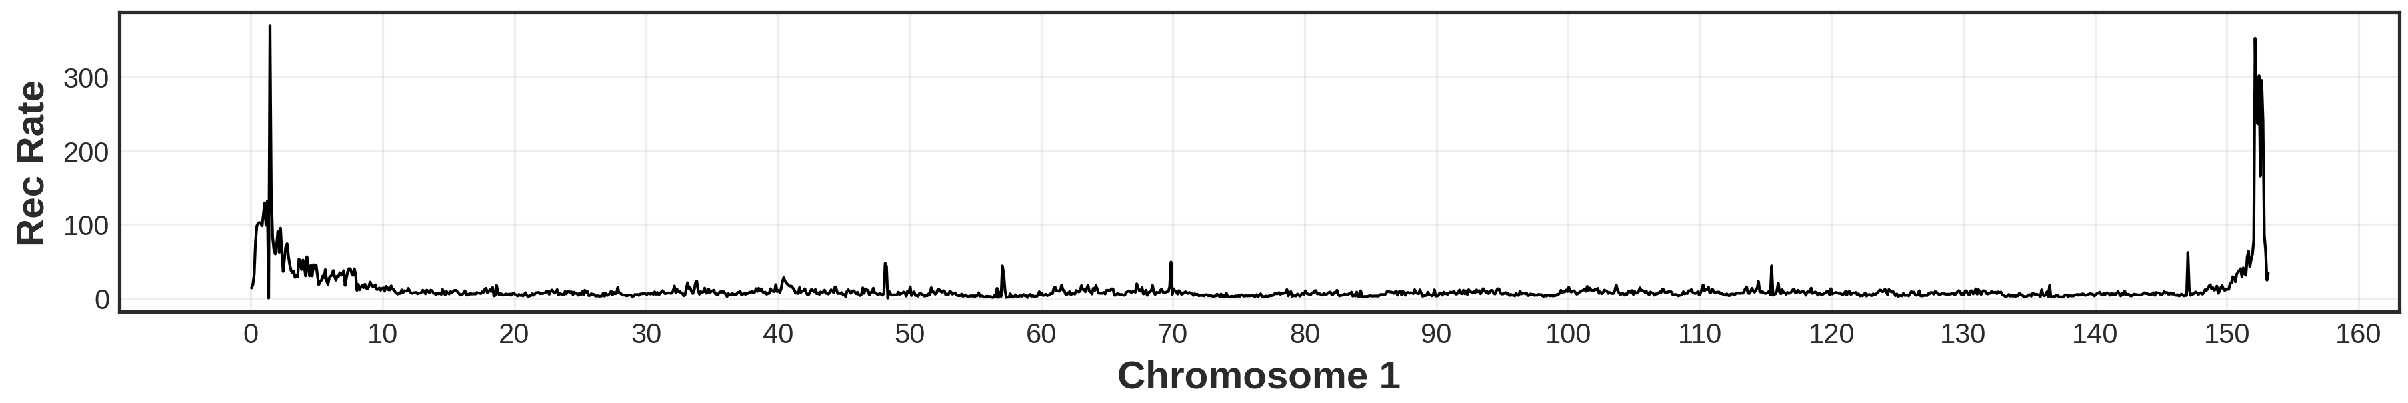
\includegraphics[width=\linewidth]{Figures/Rho_chr1.png}
		\subcaption{}
	\end{subfigure}\hfill
	\begin{subfigure}[t]{0.24\linewidth}
		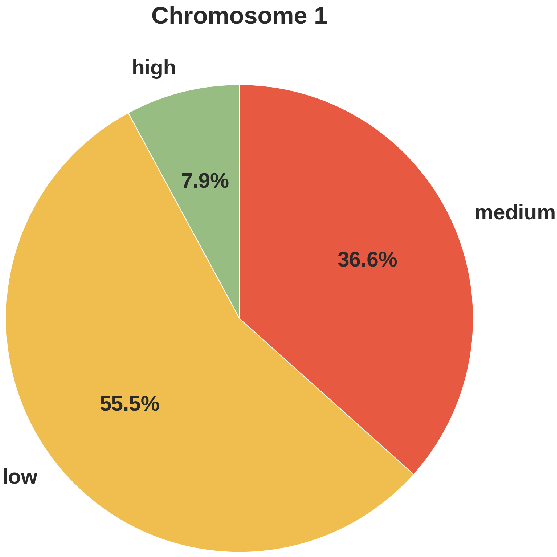
\includegraphics[width=\linewidth]{Figures/Rho_dist_chr1.png}
		\subcaption{}
	\end{subfigure}\par\medskip

	% chr10
	\begin{subfigure}[t]{0.74\linewidth}
		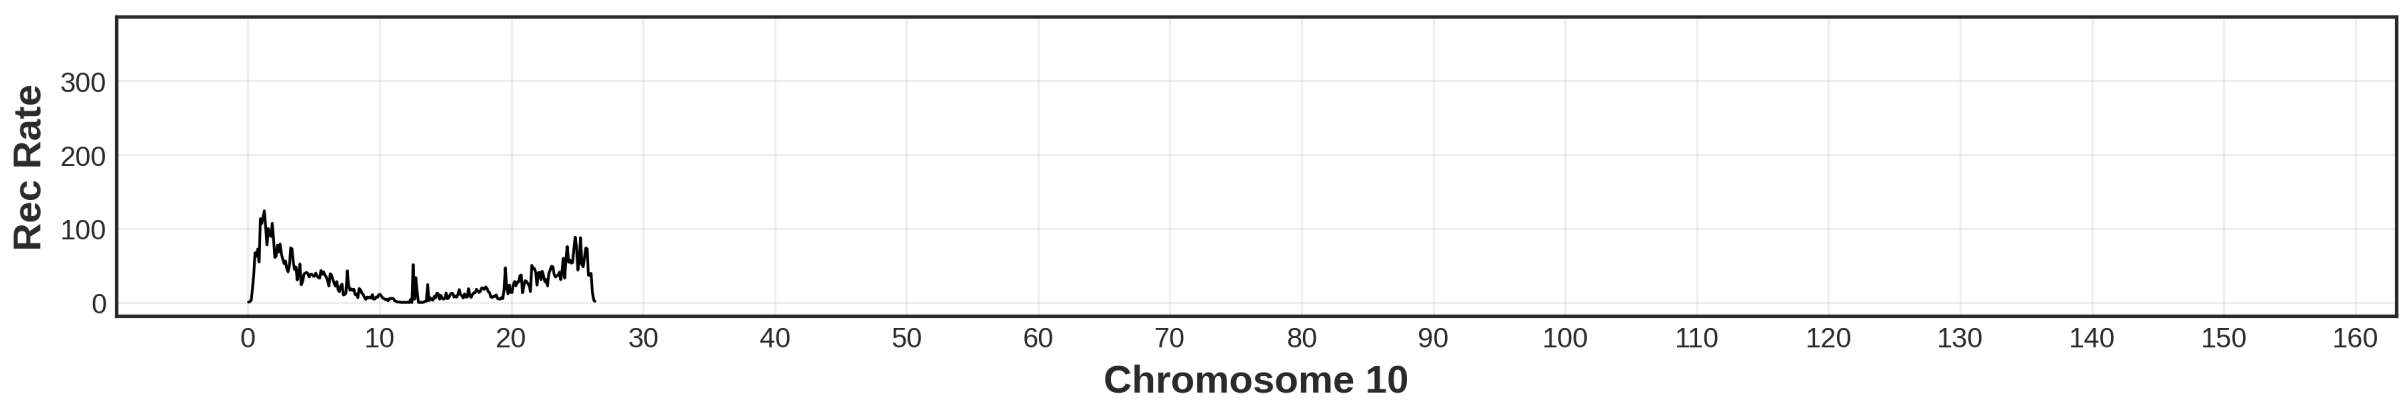
\includegraphics[width=\linewidth]{Figures/Rho_chr10.png}
		\subcaption{}
	\end{subfigure}\hfill
	\begin{subfigure}[t]{0.24\linewidth}
		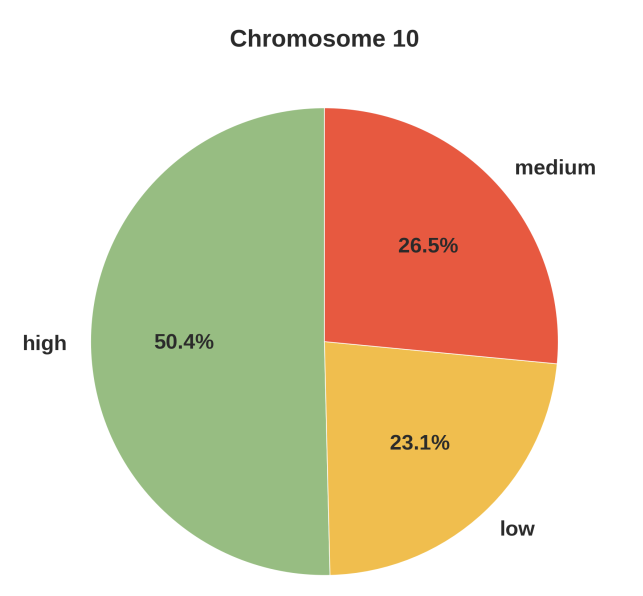
\includegraphics[width=\linewidth]{Figures/Rho_dist_chr10.png}
		\subcaption{}
	\end{subfigure}\par\medskip

	% chr30
	\begin{subfigure}[t]{0.74\linewidth}
		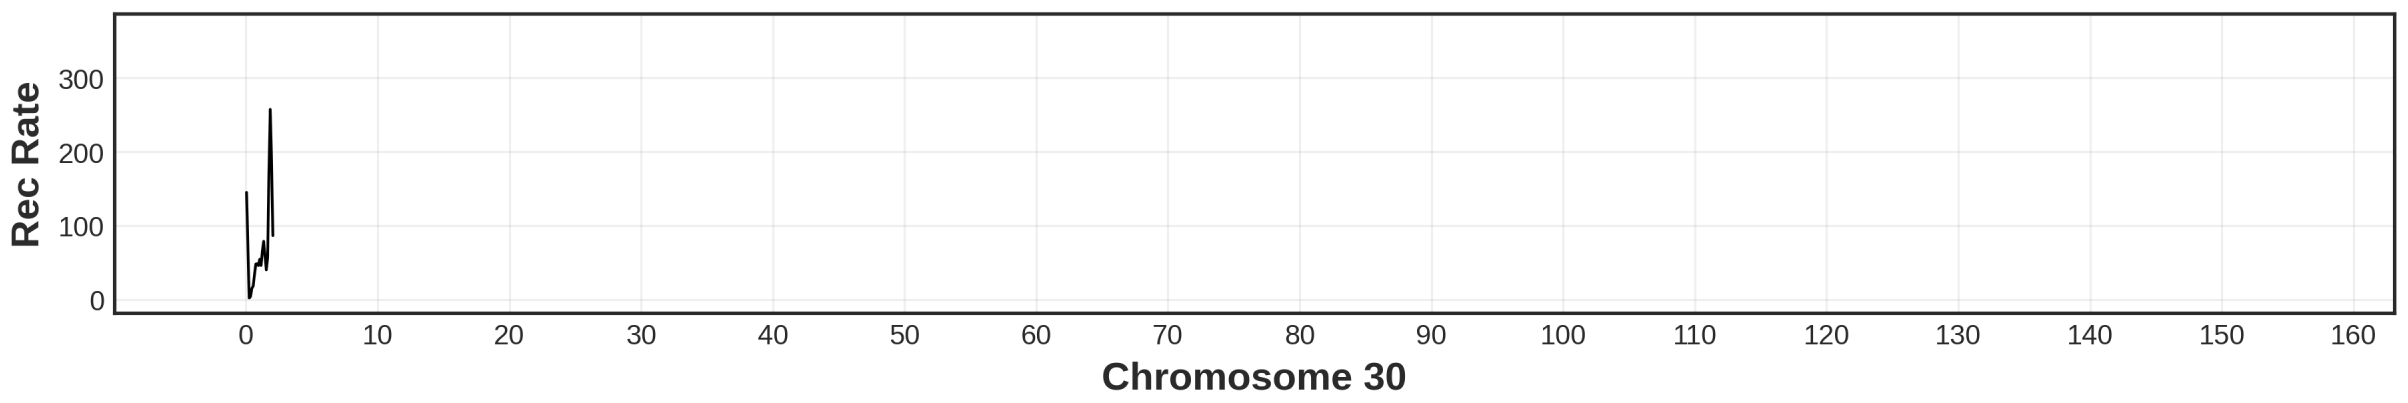
\includegraphics[width=\linewidth]{Figures/Rho_chr30.png}
		\subcaption{}
	\end{subfigure}\hfill
	\begin{subfigure}[t]{0.24\linewidth}
		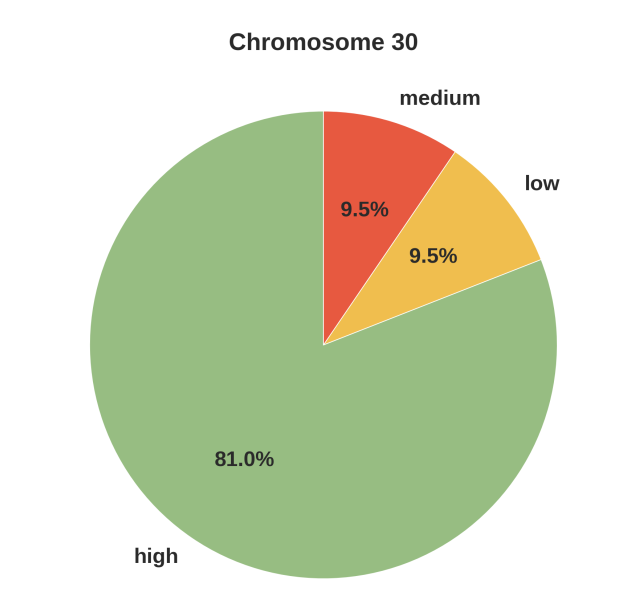
\includegraphics[width=\linewidth]{Figures/Rho_dist_chr30.png}
		\subcaption{}
	\end{subfigure}

	\caption{\textbf{a,c,e}: Recombination Rate $()\frac{cM}{Mb})$ across chromosomes 1, 10, and 30 in 100\,kb windows. \textbf{b,d,f}: Recombination Rate binned into equal tertiles (\emph{low}, \emph{medium}, \emph{high}).}
\end{figure}

\begin{figure}[htbp]
	\centering
	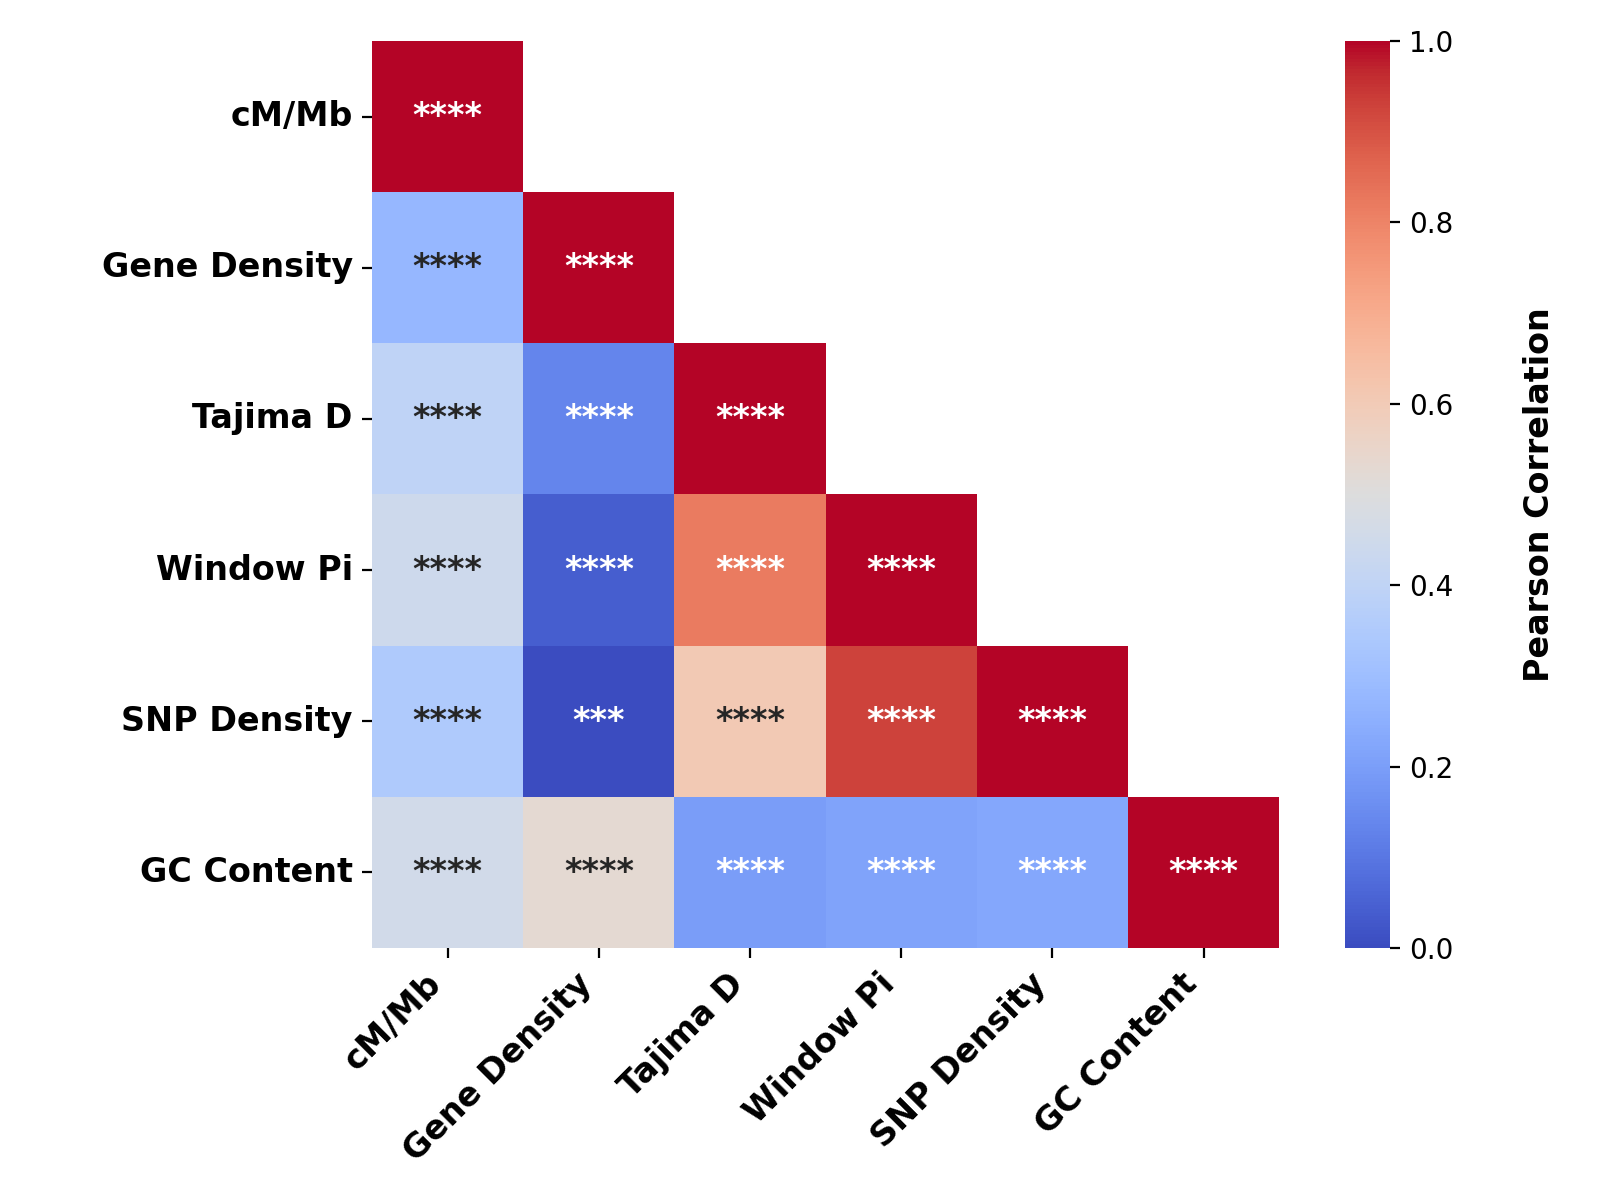
\includegraphics[width=0.50\textwidth]{../results/rec_rate_stats/feature_correlation_plot_100000.png}
	\caption{Heatmap showing the pearson correlation coefficient between several blackcap metapopulation features with corresponding \textit{p}--values. }

\end{figure}
\section{Discussion}

\section{References}

\printbibliography[heading=none]

\newpage
% ==========================
%   DECLARATION PAGE
% ==========================
\section{Declaration}
 {\large \textbf{Erklärung} \; / \; \textit{Declaration}}\\[0.8cm]

Hiermit erkläre ich, dass ich die vorliegende Arbeit selbständig und ohne
fremde Hilfe angefertigt und keine anderen als die angegebenen Quellen und
Hilfsmittel verwendet habe. Die eingereichte schriftliche Fassung der Arbeit
entspricht der auf dem elektronischen Speichermedium.\\[0.8cm]

\textit{I hereby declare that I have prepared this thesis independently and without outside
	assistance. I have not used any sources or aids other than those indicated. The submitted written
	version of the thesis corresponds to the one on the electronic storage medium.}\\[0.8cm]

Weiterhin versichere ich, dass diese Arbeit noch nicht als Abschlussarbeit an
anderer Stelle vorgelegen hat.\\[0.8cm]

\textit{Furthermore, I certify that this work has not been submitted as a thesis
	elsewhere.}\\[1.5cm]

Datum, Unterschrift\\ \textit{Date, Signature}

\end{document}

